\section{ADTool : étude de l'existant}
	\label{sec:adtool}

	ADTool est un logiciel libre permettant aux utilisateurs de modéliser des scénarios d'attaque et de défense sous la forme d'ADTrees. Il est disponible en téléchargement sur Internet (avec ou sans ses dépendances), et il existe aussi une version en ligne. Dans le but de réaliser une solution d'aide pour les expert en sécurité modélisant les ADTrees, il nous a semblé cohérent de commencer par étudier les solutions existantes. ADTool est le seul logiciel libre disponible implémentant les ADTrees : cette section détaillera ses atouts et ses points faibles.

	ADTool permet de construire des ADTrees sans difficulté. Le logiciel offre la possibilité de créer de nouveaux nœuds, d'éditer leurs labels et de leur ajouter des fils de façon simple et intuitive. Cette dernière fonctionnalité correspond à l'action \og Add Child \fg{} visible sur la {\sc Figure} \ref{fig:arbre_exemple_1}. Sur cette même figure, il est montré que les différentes actions s'effectuent de façon pratique par le biais de la souris ou de raccourcis clavier. Il est aussi possible d'ajouter des frères à un nœud choisi. Le choix des opérateurs entre ces nœuds (conjonction ou disjonction)  se fait rapidement, et la mise en place de défenses est également très facile à réaliser. 
	
	\begin{figure}[h]
        \centering
        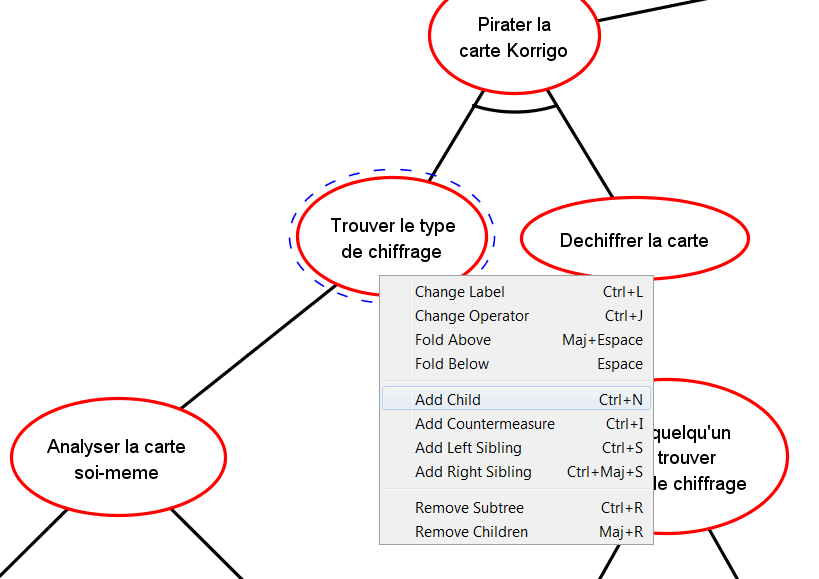
\includegraphics[width=0.8\textwidth]{figure/adtool_add_child.png}
        \caption{La création d'un arbre dans ADTool est simplifiée par des actions accessibles facilement.}
        \label{fig:arbre_exemple_1}
    \end{figure}
	
	Une fois l'arbre établi, il est possible d'ajouter des valuations à chaque feuille\footnote{Une feuille est un nœud n'ayant aucun fils.} de l'arbre selon un paramètre, qu'ADTool se charge ensuite de propager aux nœuds pères de façon récursive jusqu'à la racine. ADTool dispose à l'heure actuelle de treize paramètres de base (appelés \textit{domains}), que nous présentons dans la \textsc{Table}~\ref{tab:DescriptionParam}.
					
	\begin{table}[h]
		\centering
		\begin{tabular}{|p{6cm}|p{5cm}|}
			\hline
			\textbf{Paramètre} & \textbf{Valeurs possibles} \\
			\hline
			Difficulty for the proponent (L,M,H) & 
				Low (bas), Medium (moyen), High (élevé) ou l'infini.\\ 
			\hline
			Difficulty for the proponent (L,M,H,E) & 
				Low (bas), Medium (moyen), High (élevé), Extreme (extrême) ou l'infini.\\ 
			\hline
			Minimal cost for the proponent (not reusable) & 
				Valeurs réelles positives, ou l'infini.\\ 
			\hline
			Minimal skill level needed for the proponent & 
				Valeurs entières positives, ou l'infini.\\ 
			\hline
			Minimal time for the proponent (in parallel) & 
				Valeurs réelles positives, ou l'infini.\\ 
			\hline
			Minimal time for the proponent (sequential) (\textit{temps minimal séquentiel}) & 
				Valeurs réelles positives, ou l'infini.\\ 
			\hline
			Overall maximal power consumption & 
				Valeurs réelles positives, ou l'infini.\\ 
			\hline
			Probability of success &
				Valeurs réelles entre 0 et 1.\\ 
			\hline
			Reachability of the proponent's goal in less than k units (in parallel) & 
				Valeurs entières de 0 à k. \\ 
			\hline
			Reachability of the proponent's goal in less than k units (sequential) & 
				Valeurs entières de 0 à k. \\ 
			\hline
			Satisfiability for the opponent & 
				Vrai ou faux. \\ 
			\hline
			Satisfiability for the proponent & 
				Vrai ou faux. \\ 
			\hline
			Satisfiability of the scenario & 
				Vrai ou faux. \\
			\hline
		\end{tabular}
		\caption{Description des paramètres de base.}
		\label{tab:DescriptionParam}
	\end{table}

	\begin{figure}[h]
        \centering
        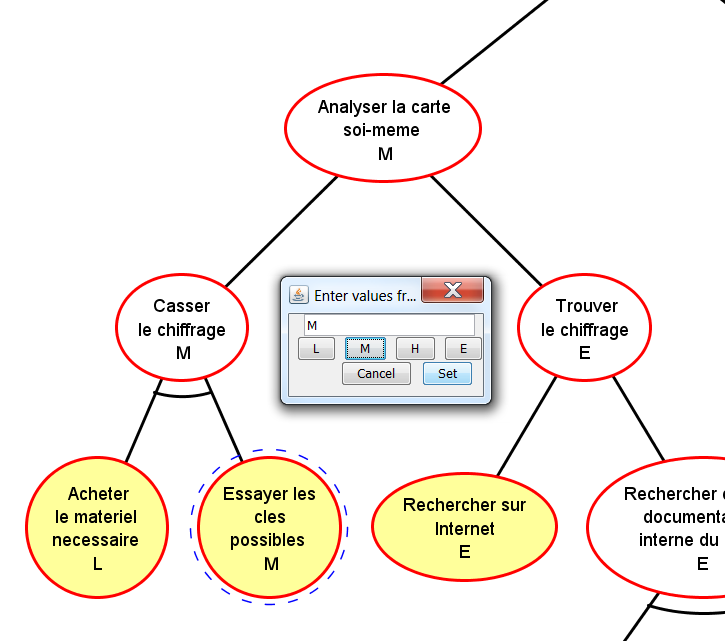
\includegraphics[width=0.8\textwidth]{figure/adtool_add_values.png}
        \caption{L'ajout de valuations aux feuilles est simple. Ces valuations se propagent ensuite récursivement à tous les antécédents.}
        \label{fig:arbre_exemple_2}
    \end{figure}
	
	Dans l'exemple de la {\sc Figure} \ref{fig:arbre_exemple_2}, chaque noeud possède une valuation selon le paramètre \og difficulté de réalisation \fg{}. Comme indiqué dans la \textsc{Table}~\ref{tab:DescriptionParam}, cette valuation peut prendre les valeurs L, M, H ou E. En éditant la difficulté de réalisation de la feuille \og essayer les clés de chiffrage possibles \fg{} à \emph{Medium}, la valuation du nœud père \og casser le chiffrage \fg{} est mise à jour automatiquement pour prendre la valeur \emph{Medium}. En effet, la difficulté de ce nœud conjonctif correspond à la difficulté la plus élevée parmi celles de ses fils. Puis, à son tour, la valuation du père de ce nœud-père est recalculée à \emph{Medium} car, étant un nœud disjonctif, sa difficulté de réalisation correspond à la difficulté la plus faible parmi celles attribuées à ses fils. L'utilisateur n'a donc pas de calcul à faire lui-même pour obtenir la valuation de la racine de son arbre, c'est-à-dire la valuation de son objectif final. 

	ADTool automatise donc la création des ADTrees et leur valuation. Mais cette étude met également en avant plusieurs limitations quant aux possibilités d'analyse pour l'utilisateur, dont voici les deux plus importantes :  

	\paragraph{Exploitation des valuations} L'utilisateur n'a aucun moyen de déterminer automatiquement le \og meilleur chemin \fg{} permettant d'atteindre la racine de l'arbre selon un paramètre donné. Il doit le trouver manuellement, en analysant la façon dont les valuations se sont propagées. Sachant qu'un arbre atteint très rapidement une taille conséquente, cette opération peut prendre beaucoup de temps et représenter un obstacle pour l'expert.

	\paragraph{Affichage des paramètres} L'analyse de l'arbre est également restreinte par le fait que la valuation d'un nœud (et donc de l'arbre entier) ne peut se faire que selon un seul paramètre à la fois. Il n'est pas possible d'afficher à la fois la \og difficulté \fg{} et le \og temps nécessaire \fg{} à la réalisation d'un nœud, par exemple. Ceci est contraignant car il est parfois difficile de séparer ces deux notions : par exemple, le nœud \og essayer les clés de chiffrage possibles \fg{} est très facile à effectuer (il suffit de taper les clés une-à-une jusqu'à trouver la bonne), mais le temps nécessaire est colossal. ADTool ne permet donc pas d'obtenir une vision complète de l'arbre par combinaison de plusieurs paramètres.

	Les deux lacunes précédentes ont été mises en avant car elles rendent l'analyse des arbres édités laborieuse. La prochaine partie détaillera l'architecture du logiciel \glasir{}, créé dans le but de dépasser les limitations évoquées.